\chaptersub{Symmetric Modes}{Private Key Cryptography}

\section{Block Ciphers}
    A \textbf{block cipher} is type of encryption based on \textbf{permutation}, where they key, $\{0,1\}^k$, defines a transposition of bits in the block to the encrypted, $\{0,1\}^b$. The block is a proportion of the message.\\
    \\
    DES was the first civilian block cipher and was developed at IBM in the 1970s. When the US government adopted it, they recommended the following four ways to use it, these are now used with any block cipher.
    \begin{itemize}
        \item Electronic Code Book
        \item Cipher Block Chaining
        \item Counter
        \item ...
    \end{itemize}
    
    \subsection{Electronic Code Book}
    This is a very simple, it \textbf{divides} the message into blocks of size $b$, pads the last one, and \textbf{encrypts them all individually}. A block cipher using ECB is only OW-CPA, as Figure~\ref{fig:ecb-attacktable} says. This the terrible!\\
    \begin{figure}[htp!]
    \centering
    \attacktable{owcpa}
    \caption{Security Models ECB passes}
    \label{fig:ecb-attacktable}
    \end{figure}
    \\
    The weakness of this mode is in the fact that the blocks of encrypted independently. This is the basis for the two attacks below, but it also means it's susceptible to \textbf{block replay}. That is where an adversary edits a bit knowing how it will affect the decrypted message. If I knew you were sending me some money, and I knew the block containing the amount you were transferring, I could change that block in the hope I would end up with a larger transaction. This could be fixed with a checksum. ECB has one positive that an error in the cipher text will not propagate to other blocks when decrypted.\\
    \\
    \textbf{Proving a cryptographic system passes a security model is beyond this scope of this course}, but you should be able to give an intuitive reason. It passes OW-CPA because, with only an encryption oracle, you would have to brute-force every possible message to match it with the ciphertext. We can always make $b$ large enough so that this is not possible.\footnote{This might be possible if you knew the context of the message, if you understand what is being sent and the domain of possible values of a block is relatively small. This is simply poor implementation of the encryption, however, and we don't worry about that.}\\
    \\
    \textbf{OW-CCA Example:} We can win an OW-CCA game by kind of cheating in the following way. If we have a decryption oracle, we can decrypt anything that is not the message. Since the blocks are independent, we can simply split the message in half and decrypt both individually and then concatenate the result.\\
    \\
    \textbf{IND-PASS Example:} In an Indistinguishability game we decide the message (of which one will be encrypted). Again we use the fact that the blocks are encrypted independently, and give one of the message as a bit string concatenated onto itself, $m_0=b_1||b_1$. The ciphertext can be split into two equal bit strings in the same way, then it was that message.
    
    
    
    \subsection{Cipher Block Chaining}
    Cipher Block Chaining removes a lot of the problems with the ECB by XORing each block with the previously encrypted block --- incorporating a dependence on the previous block. The first block of the ciphertext is called the \textbf{Initalisation Vector} (IV), and is what the first block of the message is XOR-ed with.\\
    \begin{figure}[htp!]
        \centering
        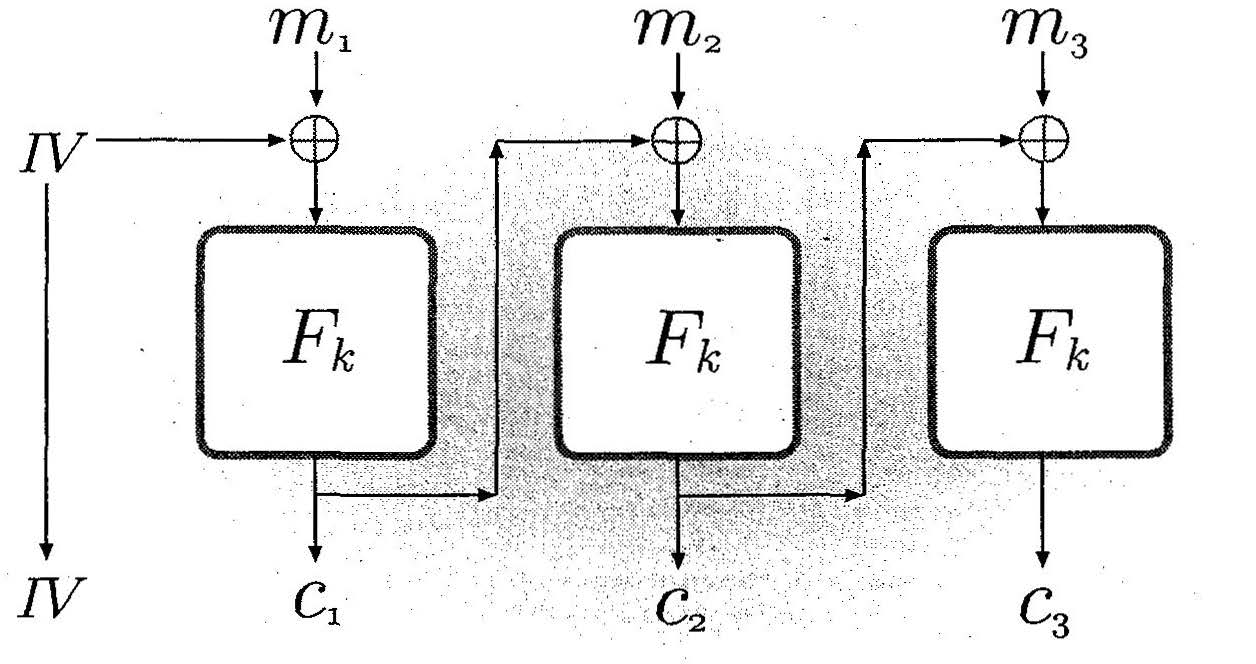
\includegraphics[width=10cm]{img/cbc}
        \caption{Diagram of CBC encrypting}
    \end{figure}
    \\
    More formally:\nopagebreak
    \begin{center}
    \begin{tabular}{lll}
    \textbf{Encryption}:                                        && \textbf{Decryption}\\
    $c_0 = IV$                                                  && $IV = c_0$\\
    $c_1 = Enc_k(m_1 \oplus IV)$                                && $m_1 = Dec_k(c_1) \oplus IV$\\
    $c_i = Enc_k(m_i \oplus c_{i-1}) \textrm{ for } i > 1$      && $m_i = Dec_k(c_i) \oplus c_{i-1} \textrm{ for } i > 1$\\
    \end{tabular}
    \end{center}
    \begin{figure}[htp!]
        \centering
        \attacktable{indcpa}
        \caption{Security of Models CBC}
        \label{fig:cbc-attacktable}
    \end{figure}
    Note that $IV$ is sent unencrypted, because it is needed for decryption. This can seem pointless, but if it is generated randomly every time, then it means that encryption is probabilistic. CBC is OW-CPA and IND-CPA but not OW-CCA or IND-CCA.\\
    \begin{figure}[htp!]
        \centering
        \begin{subfigure}[b]{0.3\textwidth}
            \centering
            
\includegraphics[width=\textwidth]{img/Tux.jpg}
            \caption{Original Image\\~}
        \end{subfigure}
        \begin{subfigure}[b]{0.3\textwidth}
            \centering
            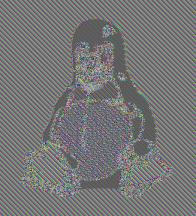
\includegraphics[width=\textwidth]{img/Tux_ecb.jpg}
            \caption{Encrypted using ECB\\~}
        \end{subfigure}
        \begin{subfigure}[b]{0.3\textwidth}
            \centering
            
\includegraphics[width=\textwidth]{img/Tux_secure.jpg}
            \caption{Encrypted using Chaining}
        \end{subfigure}
        \caption{Bitmap image of Tux being encrypted using ECB and using another method that uses chaining.}
        \label{fig:tux}
    \end{figure}
    \\
    \textbf{With a decryption oracle, CBC will fail} because of the same trick used before --- we can ask to oracle to decrypt the ciphertext with extra blocks on the end.
    
    
    
    \subsection{Counter Mode}
    Counter mode is the same as CBC mode, but 

\section{Message Authentication}
    \subsection{Why Do This}
        Encrypting data provides confidentiality (remember the three goals), but does not provide authenticity or integrity without additional sauce. This is the additional sauce.
        It comes with two flavours that are used for different things: \textbf{MDC} (Manipulation Detection Codes) and \textbf{MAC} (Message Authentication Codes). We will mainly worry about \textbf{MAC} stuff.
        The reason we use these at all is that they are the secret ingredient in getting from IND-CPA to the mythical, coveted IND-CCA level of security.


    \subsection{\textbf{M}essage \textbf{A}uthentication \textbf{C}odes, you say?}
    MAC codes are the result of hashing the message, using a hash function that takes a key.
    \begin{figure}[htp!]
        \centering
        MAC = $h_{k}(m)$
    \end{figure}

    You would then typically send the MAC concatenated at the end of the message. The hash function, as per Kerckhoff's principle, is publicly described. Given \emph{k} and \emph{m}, computing $h_{k}(m)$ should be easy.
    Given only \emph{m}, computing a correct hash should be very difficult, even if several message-to-hash pairs are already known.

    A hash function is simply a surjective mapping from arbritrarily long strings to fixed length hash strings. 

    \subsection{Security Model}
    Our security models are simple:
    \begin{itemize}
        \item \textbf{EF-PASS}: The passive attack where the bad guy can generate a valid MAC for any message, gibberish or otherwise. 
        `Existential' forgery is where the message may just be random rubbish, `Selective' forgery is creating a MAC for a specific message.

        \item \textbf{EF-CMA}: As above, but the douche of an adversary has an oracle that can perform MAC generation on other messages of his choice (but not the target message). This is the `Chosen Message' Attack
    \end{itemize}

    We will now look at two games for Existential Forgery; as a MAC may be probabilistic, we define two algorithms for these games:

    \begin{itemize}
        \item $\textbf{MAC}_{k}(m)$: Generates the MAC for message \emph{m}.
        \item $V_{k}(m, c)$: A boolean-returning verification function. True is good. False is bad. Get with the program, kids. Also this may not simply be a case of recomputing the MAC; if the algorithm that generates it is probabilistic, we need other methods of checking correctness.
    \end{itemize}

    It is a given that our opponent has access to a Verification Oracle (otherwise how will they know if they have cracked it?). 

    \begin{figure}[htp!]
    \centering
    \begin{subfigure}[b]{0.4\textwidth}
        \centering
        \begin{cryptogame}{}
            \cgameright{$V(m, c)$}
            \cgameleft{$m^{*}$, $c^{*}$}
        \end{cryptogame}
        \caption{EF-PASS: Passive Attack}
        \label{fig:ef-pass}
    \end{subfigure}
    ~
    \begin{subfigure}[b]{0.4\textwidth}
        \centering
        \begin{cryptogame}{}
            \cgameright{$V(m, c)$}
            \cgameright{$c = MAC_{k}(m)$}
            \cgameleft{$m^{*}$, $c^{*}$}
        \end{cryptogame}
        \caption{EF-CMA: Chosen Message Attack}
        \label{fig:ef-cma}
    \end{subfigure}
    \caption{MAC security games}
    \label{fig:ef-games}
\end{figure}

    There exists a `Strong Forgery' variant of \textbf{EF-CMA} called, unsuprisingly, \textbf{SF-CMA}, which changes the restriction on the MAC oracle to be that whilst $m^{*}$ can be passed to the oracle, $c^{*}$ must not have been returned.

    Assuming we can create a MAC function that achieves this, we can now make INC-CCA symmetric encryption schemes! Hooray!

    \subsection{IND-CCA Here We Come}
    The reason that CBC and CTR modes, whilst groovy, were not \textbf{IND-CCA} was that an attacker could look at our ciphertext and construct a related one which could be decrypted through their oracle, giving them a related plaintext.

    MAC prevents them from doing that! Sweet! So to make an \textbf{IND-CCA} secure scheme you will need:
    \begin{itemize}
        \item One \textbf{IND-CPA} secure symmetric cipher \emph{E}.
        \item One \emph{SECURE}\footnote{i.e. Cannot produce a valid \textbf{MAC} without access to the correct key} \textbf{MAC} function \emph{MAC}.
        \item One hybrid key consisting of $k_{0}$ and $k_{1}$ which are the keys for \emph{E} and \emph{MAC} respectively.
    \end{itemize}

    We can then construct encryption and decryption thusly:
    \begin{figure}[htp!]
    \centering
    \raisebox{-0.5\height}{
        \begin{subfigure}[b]{0.4\textwidth}
            \centering
            \textbf{Encrypt}
            \begin{enumerate}
                \item Split $k$ into $k_{0}$ and $k_{1}$
                \item $c_{0} = E_{k_{0}}(m)$
                \item $c_{1} = MAC_{k_{1}}(c_{0})$
                \item And voila: $c = (c_{0}, c_{1})$
            \end{enumerate}
            \label{fig:ind-cca-enc}
        \end{subfigure}
        }
    ~
    \raisebox{-0.5\height}{
        \begin{subfigure}[b]{0.4\textwidth}
            \centering
            \textbf{Decrypt}
            \begin{enumerate}
                \item Split $k$ into $k_{0}$ and $k_{1}$
                \item Split $c$ into $c_{0}$ and $c_{1}$
                \item $c_{1}^{*} = MAC_{k_{1}}(c_{0})$
                \item If $c_{1}^{*} \neq c_{1}$ then ABORT and return $\bot$
                \item Else return $m$ where $m = D_{k_{0}}(c_{0})$ 
            \end{enumerate}
            \label{fig:ind-cca-dec}
        \end{subfigure}
    }
    \caption{How To Make an IND-CCA Scheme}
    \label{fig:ind-cca-ed}
    \end{figure}

    This obviously involves the ciphertext being expanded (more than it might be already) because it includes a MAC. 

    With the MAC allowing us to validate a ciphertext as being `authentic', this type of scheme is often called \emph{`authenticated encryption'}.
    It is important to realise the \textbf{very important} distinction between this idea, which is that a ciphertext is authentic, and the concept that a ciphertext came from where it was supposed to, which is part of the regular cryptographic definition of `Authenticity'.

    \subsection{How To Make A MAC}
    There are a few types of MAC schemes, from MACs that are custom made for that specific encryption scheme to MACs that are derived from MDCs (Manipulation Detection Codes).

    The most popular, and exceedingly examinable, variants that we look at are all based on CBC-mode block ciphers. They are covered by various international standards\footnote{Gotta love standards. Thrilling stuff} and are very widely used. We shall refer to schemes like this under the title of CBC-MAC. Like this...

    \subsection{CBC-MAC}
    CBC-MAC is pretty much a straightforward application of a block cipher (like DES or AES). We just have to add the MAC on after padding the ciphertext.

    Given our cipher, which operates on blocks of \emph{b} bits, we can make a MAC really simply; assuming we have \emph{q} data blocks in our message, $m_{1}, m_{2}...m_{q}$, we would do as follows:
    \begin{enumerate}
        \item Set initial intermediate variables: $I_{1} = m_{1}, O_{1} = e_{k}(I_{1})$
        \item For $i = 2, 3 ... q$:
            \begin{itemize}
                \item $I_{i} = m_{i} \oplus O_{i - 1}$
                \item $O_{i} = e_{k}(I_{i})$
            \end{itemize}
        \item Do any post-processing you want on $O_{q}$.
        \item Truncate if necessary to $m$ bits and serve piping hot.
    \end{enumerate}

    In terms of padding the ciphertext, there are 3 schemes suggested in those groovy groovy standards. All of these pad to a whole number of blocks.
    \begin{itemize}
        \item Just add zeroes. Easy, right?
        \item Add a single 1, then trail out with zeroes.
        \item Pad with zeroes until you get a whole number of blocks, then add a block containing the length of the unpadded message.
    \end{itemize}

    In terms of optional post-processing, there are two specified methods:
    \begin{itemize}
        \item Choose another key, $k_{1}$, and replace $O_{q}$ with $e_{k}(d_{k_{1}}(O_{q})$
        \item Choose another key, $k_{1}$, and replace $O_{q}$ with $e_{k_{1}}(O_{q})$ 
    \end{itemize}

    Either one of those can make it much harder to do a brute force search for $k$. Which is a good thing, young padawan. Oh yes.

    \subsection{Hashing}
    Like we said, hashing in this case is just an efficient function mapping arbritrarily long binary strings to fixed length binary strings. Simples.

    Incidentally, these hashes are essentially MCDs, though they are not called that now. Used to be the case that you'd do a hash (MDC), concatenate it to the message and then encrypt that. The problem with a concatenate-then-encrypt scheme under CBC is that an attacker can create a message that consists of the message they wish to send, a hash for it, and then some other random guff, and then hash that (this is an CPA method). If the attack then truncates the resulting ciphertext they get their valid target ciphertext, complete with hash. TODO: EXPLAIN THIS BETTER DRUMMOND YOU CRAZY MAN.

    I know that earlier I talked about hashing with a key, but in practice hash functions don't have a key. It is often simpler to consider a family of functions, and require three conditions of them:
    \begin{enumerate}
        \item Preimage Resistance: given $c = h(m)$, hard to find another $m^{'}$ such that $h(m^{'} = c = h(m)$
        \item 2nd Preimage Resistance: The same as preimage resistance, except that we are also given $m$.
        \item Collision Resistance: hard to find $m, m^{'} \neq m$ such that $h(m) = h(m^{'}$
    \end{enumerate}

    Typical practical choices for a cryptographic hash are the SHA family, or the RIPEMD family.

    \subsection{From Hash To MAC}

    Given a hash function, how can we bung a key in there sensibly? There are the simple prefix, suffix and envelope methods, though these are not secure.
    \begin{itemize}
        \item With prefixing it is possible to calculate $MAC_{k}(m||m^{'})$ without knowing the key. Simply split your intended message in half, and you're good to go. Exact method not shown in notes.
        \item Suffixing suffers from a weakness that makes it easier to find collisions in the hash function; this can be done offline, as well, so you do not need to send lots of queries to the target. Exact methodology not disclosed in notes.
        \item Envelope method with padding: The reason this isn't secure isn't given in the notes, and I can't find it online. TODO: SOMEONE HELP ME OH GOD PLEASE
    \end{itemize}

    It is better to use HMAC (keyed-\textbf{H}ash \textbf{M}essage \textbf{A}uthentication \textbf{C}ode):

    $$HMAC_{k}(m) = h(k||p_{1}||h(k||p_{2}||m))$$

    Where $p_{1}$ and $p_{2}$ are fixed strings used to pad $k$ to a full block.

    You can use both MDC and MAC for data integrity, with or without confidentiality.

    Without confidentiality:
    \begin{itemize}
        \item \textbf{MAC}: compute $MAC_{k}(m)$ and send $m||MAC_{k}(m)$
        \item \textbf{MDC}: Send h(m) over a seperate, authenticated channel.
    \end{itemize}

    With confidentiality:
    \begin{itemize}
        \item \textbf{MAC}: need two different keys, $k_{1}$ and $k_{2}$
        \begin{itemize}
            \item $k_{1}$ is for computing $c = e_{k_{1}}(m)$
            \item $k_{2}$ if for computing $MAC_{k_{2}}(c)$, which you append to $c$ before sending that combined string.
        \end{itemize}
        \item \textbf{MDC}: we only need one key $k$ for encryption, where we send $c = e_{k}(m||h(m))$, but as we discussed earlier this can be compromised by a man in the middle attack.
    \end{itemize} 